\chapter{А на бумаге записать можно? Ноты, табы}
\label{ch:notes}

Нотную запись нельзя назвать эталоном простоты. Она, несомненно, сложнее, чем могла бы быть. Так уж сложилось.

Уважая гениальность предков, мы изучим её такой, какая она есть, и постораемся понять почему она такая.

% TODO:
%\begin{figure}[!ht]
%    \centering
%    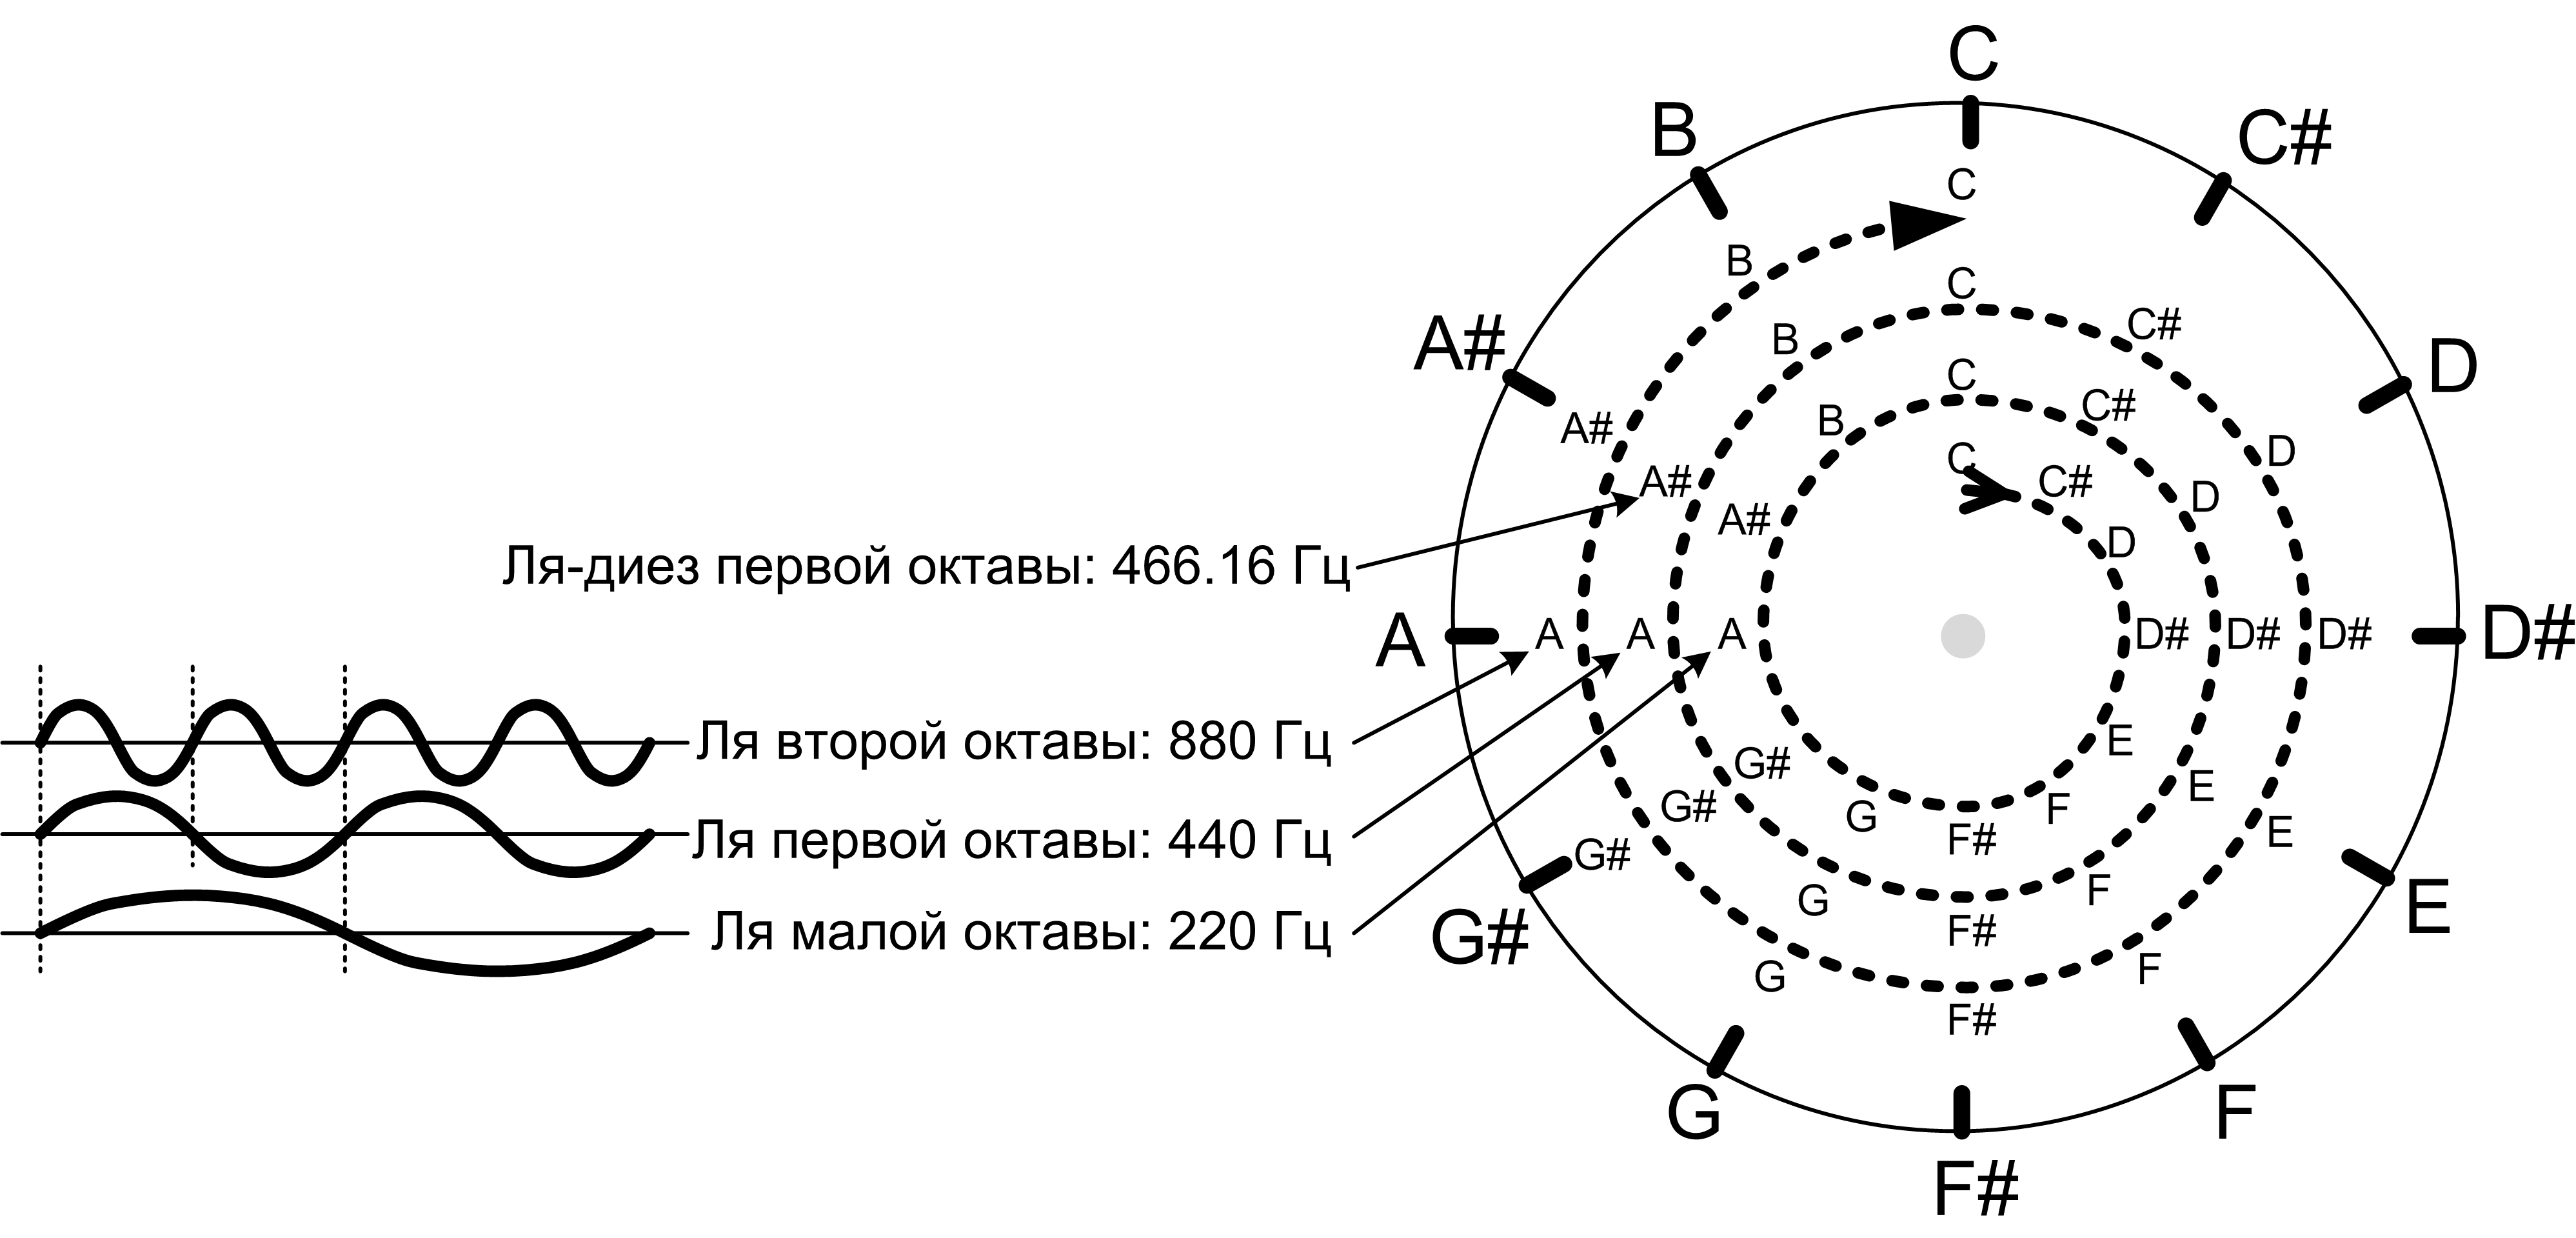
\includegraphics{fig/intervals/octave-spiral} 
%    \caption{Цикличность музыкальных звуков}\label{fig:music:tone:octave}
%\end{figure} 
%
%ЛЯ-диез первой октавы, который на полутон выше эталонного ЛЯ, имеет частоту $440\cdot\sqrt[12]{2}\approx 466,16$ герц. Эти различия ощущаются на слух. Звук СИ первой октавы (два полутона от эталонного ЛЯ) имеет частоту $440\cdot(\sqrt[12]{2})^2\approx 493,88$. И так далее, например, ЛЯ второй октавы (на 12 полутонов, то есть не октаву выше эталонного) имеет, как и положено, в два раза большую частоту: $440\cdot(\sqrt[12]{2})^{12}=440\cdot 2=880$ Гц. Ряд музыкальных звуков по спирали <<наматывается>> на октаву (см. рисунок\footnote{Забегая немного вперед (иначе рисунок трудно понять), скажем, что гитаристы чаще обозначают ноты латинскими буквами: ДО(С), РЕ(D), МИ(E), ФА(F), СОЛЬ(G), ЛЯ(A), СИ(B). ЛЯ-диез, соответственно: A\#} \ref{fig:music:tone:octave}).


\section{А словами как назвать? Названия нот}
\label{ch:notes:names}

\emph{Нота} --- это \emph{буква} (знак) музыкального письма, позволяющая определить \emph{высоту} (частоту колебаний) и \emph{длительность} музыкального звука. 

В Русской традиции принято использовать следующие \emph{семь} названий нот, которые приведены в порядке возрастания частоты колебаний (высоты звука): 
\begin{center}
    ДО, РЕ, МИ, ФА, СОЛЬ, ЛЯ, СИ. 
\end{center}

Многие знают эту последовательность нот как детский стишок\footnote{Такие названия нот удобны тем, что их можно \emph{петь}. Тянуть последнюю гласную пока воздуха хватает! Человеку на самом деле не нужна гитара! Музыкальный инструмент всегда с собой --- голос. Друзья, поверьте, есть такие люди, которые могут петь по нотам. Их мало на нашей эстраде, но они есть! Только не надо думать, что если вы споете, например, ДО-О-О-О, то это прозвучит в унисон с пятой струной на третьем ладу. Фигушки. Не льстите себе. Такое может сделать только мастер. Он любую гласную вытянет в унисон с любым сыгранным не гитаре звуком!}. Эти ноты составляют октаву (и правда, чуть позже об октавах!).

Американцы и англичане называют ноты не как мы, а буквами латинского алфавита: 
\begin{center}
    A(ля), B(си), C(до), D(ре), E(ми), F(фа), G(соль).
\end{center}

И жили они, не тужили, с октавой, начинающейся с ЛЯ\ldots Ага, вроде всё логично и просто, как азбука\footnote{Латинские алфавит читается: A-эй, B-би, C-си, D-ди, E-и, F-эф, G-джи, H-эйч}. Как вдруг, в результате спонтанного шизоидного сдвига, всем вдруг стало ясно, что октава должна начинаться с ДО\footnote{Причина сего интересна не только психиатрам! Если вы разберетесь с \emph{музыкальным ладом}, то вы сами дадите этому заскоку рациональное объяснение}! И стало: CDEFGAB. А потом кому-то покорзилось, что для ноты СИ буквы не хватило! И назначили для ноты СИ очередную свободную латинскую букву H! Гитаристам с латиницей дело иметь придется часто, поэтому запомните приведенное соответствие и будьте готовы к тому, что для обозначения ноты СИ может быть использована латинская буква H\footnote{Все даже чуть сложнее. Если вы увидели книжку, где используется H, то знайте, что это СИ. Но не падайте в обморок, если вдруг увидите, что используется и латинская B. В данном клиническом случае B будет обозначать ноту CИ-бемоль!}.

Нота звучит \emph{выше}, если частота колебаний струны \emph{больше}. Ну а низкая нота --- это колебания с малой частотой. Например, в соответствии с международным стандартом, струна, звучащая на ноте Ля первой октавы (об октавах скажу позже) колеблется с частотой 440 герц, то есть совершает 440 полных колебаний в секунду\footnote{Допускается вольность принять за Ля первой октавы любую частоту из интервала от 430 до 450 герц. Многие фанатики утверждают, что Ля в 432 Гц одобрена Богом (и оздоравливающе действует на организм), а стандартизированная 440 Гц --- от Сатаны (и разрушает психику)}.

Допустим, с названиями нот все понятно\ldots Так что получается, музыкальных звуков всего семь? Конечно нет! Пусть мы дошли до последней ноты СИ и... И текущая \emph{октава} кончилась. Но началась следующая! В следующей октаве все повторится: ДО, РЕ, МИ, ФА, СОЛЬ, ЛЯ, СИ. Только вот частота звука для соотвествующей ноты будет в \emph{два} раза больше! То есть, например, ноте Ля второй октавы соответствует вдвое большая частота (880 Гц), чем ноте Ля первой октавы (стандартные 440 Гц).

Октавы, использующиеся в музыке, имеют следующие названия.
\begin{center}
    \begin{tabular}{ll}
        \hline\hline
        Название октавы         & Частота ноты Ля, Гц \\
        \hline\hline
        
        Субконтроктава          & 27.5 \\
        Контроктава             & 55   \\
        \emph{Большая октава}   & 110  \\
        \emph{Малая октава}     & 220  \\
        \emph{Первая октава}    & \fbox{440}  \\
        \emph{Вторая октава}    & 880  \\
        Третья октава           & 1760 \\
        Четвертая октава        & 3520 \\
        Пятая октава            & 7040 \\
        \hline
    \end{tabular}
\end{center}

В таблице \emph{выделены} те октавы, которые входят в диапазон шестиструнной гитары. Справедливости ради следует сказать, диапазон звучания шестиструнной гитары полностью включает лишь малую и первую октавы.

А вот теперь пришло время для секретов: традиционно в октаве принято выделять \emph{двенадцать} звуков! 

Погодите, погодите, скажете вы: <<До, Ре, Ми, Фа, Соль, Ля, Си>> --- семь нот! И октава названа, вероятно, не просто так: <<octo>> --- это восемь, восьмая нота\footnote{Почему октава названа октавой см. в разделе \ref{sec:harmony:interval}. На самом деле октава --- это определенное расстояние между звуками}! Все логично!

Люди в шоке, но молчат! <<До, Ре, Ми,\ldots>> --- это \emph{названия} лишь семи звуков из 12, составляющих октаву. (12-7)=5 звуков не удостоились отдельных имен. Итак, оставшиеся 5 звуков находятся между:
\begin{enumerate}
    \item ДО и РЕ (этот звук может быть назван либо ДО-диез, либо РЕ-бемоль)
    \item РЕ и МИ (РЕ-диез или МИ-бемоль)
    \item ФА и СОЛЬ (ФА-диез или СОЛЬ-бемоль)
    \item СОЛЬ и ЛЯ (СОЛЬ-диез или ЛЯ-бемоль)
    \item ЛЯ и СИ (ЛЯ-диез или СИ-бемоль)
\end{enumerate}    

Как видно, эти <<промежуточные>> ноты могут называться двояко. Какое из имен выбрать? Постараюсь ответить кратко: если вы читаете этот текст и узнаёте для себя что-то новое, то вам позволительно использовать любое\footnote{Это как грамотность в Русском языке: надеть или одеть? Одеть Надежду, надеть одежду! Чужак не осилит. Так что называйте как хотите, знающие друзья поправят, если что. Только помалкивайте на какой-нибудь музыкальной конференции в кругу маститых классических исполнителей}! Все 12 звуков октавы в порядке увеличения высоты:
\begin{center}
    ДО, \emph{ДО-диез}, РЕ, \emph{РЕ-диез}, МИ, ФА, \emph{ФА-диез}, СОЛЬ, \emph{СОЛЬ-диез}, ЛЯ, \emph{ЛЯ-диез}, СИ
\end{center}

Отметим, что между МИ и ФА, а также между СИ и ДО, промежуточных звуков нет\footnote{Вам уже давно хочется сказать: <<Какого черта?>>. Почему? Зачем эти сложности? Друзья мои, болею за вас! Творится полный беспредел с точки зрения кодирования. Можно проще, но все привыкли. Традиция}.

В учебниках говорится, что добавление суффикса <<диез>> означает повышение частоты исходной ноты на <<полутон>>, что математически соответствует увеличению частоты в $\sqrt[12]{2}$ раз. И это в целом правильно, только обычно ученики начинают думать, что между соседними нотами из списка ДО, РЕ, МИ, ФА, СОЛЬ, ЛЯ, СИ --- расстояние в два <<полутона>> (то есть в <<тон>>)! Не забыайте, что между нотами МИ и ФА, а также между СИ и ДО <<промежуточных>> нот нет и расстояние между ними --- один <<полутон>>. 

Как видно из реальной последовательности, следуя такой логике, например, МИ-диез --- это ФА, или СИ-диез --- это ДО следующей октавы. Обычно ноту ФА, конечно никто не называет МИ-диез --- это оскорбительно, но никто и не запрещает так делать. 

То же самое можно сказать и о суффиксе <<бемоль>>, он понижает ноту на полутон. И, например, До-диез, это тот же звук, что и РЕ-бемоль. А если вы хотите оскорбить ноту МИ, то назовите её ФА-бемоль. Если вы хотите назвать все 12 звуков октавы в обратном порядке, то грамотно будет использовать суффикс <<бемоль>>, а не <<диез>>:

\begin{center}
СИ, СИ-бемоль, ЛЯ, ЛЯ-бемоль, СОЛЬ, СОЛЬ-бемоль, ФА, МИ, МИ-бемоль, РЕ, РЕ-бемоль, ДО.
\end{center}


\section{Что тут зашифровано? Запись нот}

Чтобы записать ноты, купите нотную тетрадь или на обычном листе начертите нотоносец --- пять параллельных, расположенных друг под другом через равные интервалы (около двух миллиметров) линий:
 

Традиционно ноты для шестиструнной гитаре записываются в скрипичном ключе, который своим хвостиком огибает вторую снизу линию нотоносца, на которой располагется СОЛЬ \emph{малой} октавы\footnote{Для других музыкальных инструментов, в первую очередь, для фортепиано, скрипичный ключ показывает положение СОЛЬ \emph{первой} октавы, но для гитары, чтобы использовать один нотоносец, ноты пишут на <<фортепианный>> скрипичный нотоносец на октаву выше.}.

\section{Как это сыграть на гитаре? Гитарная табулатура}



%TODO ритм и переборы